\section{Entity-Resolution}
\label{sec:approaches}

Zwei eigentlich identische Objekte können sich durch verschiedene Schreibweisen,
Abkürzungen, oder der Verwendung unterschiedlicher Persistierungen unterscheiden.
So können z.B. die beiden Instanzen \glqq Peter Müller\grqq und \glqq Peter Mueller\grqq die selbe Person darstellen,
obwohl sie unterschiedlich geschrieben sind.

Ziel der Entity-Resolution ist es durch automatische Verfahren herauszufinden,
ob zwei Instanzen aus verschiedenen Datensätzen dasselbe Objekt in der realen Welt repräsentieren.
Das ist z.B. nötig, wenn man verschiedene Datenquellen zusammenführen oder eine Datenbereinigung vornehmen möchte.
Dazu ist es nötig, geeignete Methoden zu verwenden bzw. zu entwickeln,
welche identische Instanzen möglichst schnell und genau identifizieren können.
Im folgenden sollen zwei Verfahren vorgestellt und in der weiteren Arbeit verglichen werden.

\subsection{Entity-Resolution mit N-Grammen}
\label{sec:approaches:n-gramm}

Für die Berechnung von Ähnlichkeiten mittels N-Grammen müssen aus den zu vergleichenden Instanzen zuerst N-Gramme erzeugt werden.
Beispielsweise werden aus den beiden Instanzen \glqq Peter Müller\grqq und \glqq Peter Mueller\grqq die folgenden Trigramme erzeugt:
\input{n-gramms.conf}

Mittels der Jaccard-Ähnlichkeit kann nun die Ähnlichkeit von A und B berechnet werden:

$Jaccard(A, B)$ $=$ $\frac{A \cap B}{A \cup B}$ $=$ $\frac{5}{10}$ $=$ $\frac{1}{2}$

Wenn man nun einen Schwellwert festlegt und die berechnete Ähnlichkeit ist größer oder gleich diesem Schwellwert,
so geht man davon aus, das es sich um die selben Instanzen handelt.

\subsection{Entity-Resolution mit N-Grammen unter Verwendung von Bloom-Filtern}
\label{sec:approaches:bloom}

Eine zentrale Rolle bezüglich der Performance der Entity-Resolution stellt der Aufwand für die Bestimmung der Ähnlichkeit zweier Objekte dar.
Insbesondere ein wie oben vorgestellter Ansatz, der auf der Berechnung des Jaccard-Index zwischen Mengen basiert,
ist aufgrund teurer Schnitt- und Vereinigungs-Berechnungen aufwändig.
Ein alternativer Ansatz stellt eine approximative Lösung, zum Beispiel unter Verwendung von Bloom-Filtern, dar.

\subsubsection{Bloom-Filter}

Ein Bloom-Filter ist eine Datenstruktur, die effizient - aber dafür approximativ - entscheidet,
ob ein beliebiges Element in einer, durch den Bloom-Filter repräsentierten, Menge enthalten ist.
Für einen Bloom-Filter $A_{BF}$ einer Menge $A$ gilt dabei stets: $x \in A$ $\Rightarrow$ $x \in A_{BF}$.

Realisiert wird ein solches Objekt mit einem Bit-Array der Länge $n$,
sowie einer Anzahl $k$ unterschiedlicher Hashfunktionen.
Diese Hashfunktionen haben jeweils einen Wertebereich von $0$ bis $n - 1$.
Initial ist der Bit-Array mit Nullen gefüllt.

Anschließen werden die Elemente der verwalteten Menge eingefügt.
Dazu werden mittels der $k$ verschiedenen Hashfunktionen $k$ Hashwerte ermittelt.
Jeder dieser Hashwerte wird nun auf die entsprechende Position im Bit-Array übertragen.
Dazu werden diese Positionen auf $1$ gesetzt.
Wenn eine Position schon durch einen anderen Hashwert auf $1$ gesetzt worden ist,
kommt es zu einer Kollision und diese Position wird auf $1$ belassen.

\begin{wrapfigure}{O}{.49\textwidth}
	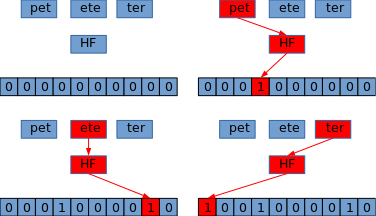
\includegraphics[width=.48\textwidth]{bloom_filter_example_insert.png}
	\caption{Einfügen vom Trigrammen in einen Bloom-Filter}
	\label{fig:add_bf}
	\vspace*{-0.4cm}
\end{wrapfigure}

Um zu überprüfen, ob ein bestimmtes Element im Bloom-Filter enthalten ist, berechnet man seine $k$ Hashwerte.
Ist an einer der $k$ Stellen im Bit-Array eine $0$, so ist dieses Element nicht in der Menge enthalten.
Steht jedoch an allen Positionen eine $1$, so ist der Wert mit einer hohen Wahrscheinlichkeit in der vom Bloom-Filter repräsentierten Menge enthalten.
Aufgrund möglicher Kollisionen kann man im Allgemeinen weder exakt bestimmen,
wie viele disjunkte Elemente ein Bloom-Filter beherbergt, noch sicher sagen, dass ein Element wirklich enthalten ist.

\refnice{Abbildung}{fig:add_bf} visualisiert das Einfügen der Trigramme des Wortes \glqq Peter\grqq.
Es wird veranschaulicht, wie das zuerst leere Bit-Array nach und nach gefüllt wird.
Zur Vereinfachung wird nur eine Hashfunktion verwendet.

\subsubsection{Einsatzszenario in der Entity-Resolution}

Ein Bloom-Filter ist unter den oben beschriebenen Eigenschaften in der Lage, eine Menge zu repräsentieren.
Des weiteren lässt sich ein logisches UND beziehungsweise ein logisches ODER zwischen den Bit-Arrays,
die den Kern einer jeden solchen Datenstrukturen bilden, extrem performant bilden.
Dieser Gedanke führt zu der zentralen Fragestellung dieses Praktikums:\\
Lässt sich die Berechnung der Jaccard-Ähnlichkeit zwischen zwei Mengen durch den Einsatz von Bloom-Filtern
optimieren? Wenn ja, zu welchem Preis?\\

Anschaulich betrachtet bedeutet dies, dass für zwei Mengen $A$ und $B$ - mit entsprechenden Bloom-Filtern $A_{BF}$ bzw.
$B_{BF}$ - der Jaccard-Index gegeben ist durch:

$Jaccard(A_{BF}, B_{BF})$ $=$ $\frac{|A_{BF} \wedge B_{BF}|}{|A_{BF} \vee B_{BF}|}$ $=$
$\frac{\text{geschätzte Anzahl Elemente in } A_{BF} \wedge B_{BF}}{\text{geschätzte Anzahl Elemente in } A_{BF} \vee B_{BF}}$\\
\begin{wrapfigure}{O}{.49\textwidth}
	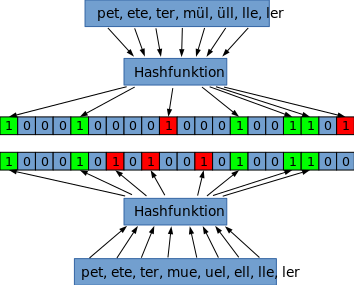
\includegraphics[width=.48\textwidth]{bloom_filter_vergleich.png}
	\caption{Vergleich mit Bloom-Filtern}
	\label{fig:sim_bf}
	\vspace*{-2cm}
\end{wrapfigure}

\refnice{Abbildung}{fig:sim_bf} zeigt diese Funktionsweise für die Berechnung der Ähnlichkeit mittels Bloom-Filtern.
Dabei werden die beiden Instanzen \glqq Peter Müller\grqq~und \glqq Peter Mueller\grqq~vergleichen.
Wenn man beide Bit-Arrays vergleicht, sieht man,
das die Anzahl der UND's gleich 5 und die Anzahl der OR's gleich 10 ist.
Dementsprechend würde die Jaccard-Ähnlichkeit $\frac{5}{10}$ entsprechen.

\newpage
\subsubsection{Gefahren beim Einsatz eines Bloom-Filters}

Für eine approximative Lösung des Entity-Resolution-Problems über den vorgestellten Bloom-Filter-Ansatz
wäre es vorteilhaft, wenn eine allgemeine Beziehung des Jaccard-Indizes für Mengen zu denen mit
Bloom-Filtern existiert.
Insbesondere ein Bezug wie $Jaccard(A, B)$ $\leq$ $Jaccard(A_{BF}, B_{BF})$ wäre wünschenswert.

Leider existieren im Allgemeinen keine derartigen Beziehungen.
Als Ursachen dafür können Kollisionen an verschiedenen Stellen im Workflow identifiziert werden.\\
So bewirken diese beim Aufbau eines Bloom-Filters, dass eine später repräsentierte
Vereinigung kleiner, und der Schnitt größer wird.
Dem entgegen bewirken Kollisionen bei der Bildung der Vereinigung von Bloom-Filtern (logisches oder) eine
unberechtigte Vergrößerung der Mächtigkeit der Vereinigung, während bei dem Schnitt (logisches und)
keine derartigen Effekte auftreten.
